\documentclass{article}
\usepackage[utf8]{inputenc}
\usepackage[english]{babel}
\usepackage{amsmath}
\usepackage{amssymb}
\usepackage{graphicx}
\usepackage{listings}
\usepackage{color}
\usepackage{amsthm}
\usepackage{babel} 
\graphicspath{ {./images/} }
% \includegraphics{sun}

\newtheorem{theorem}{Theorem}
\newenvironment{amatrix}[1]{%
  \left(\begin{array}{@{}*{#1}{c}|c@{}}
}{%
  \end{array}\right)
}
% \newlist{background}
% \setlist[background]{
%   label = \textbf{Background \arabic*.}, 
%   wide
% }


\renewcommand{\qedsymbol}{Q.E.D.}
\newcommand{\norm}[1]{\left\lVert#1\right\rVert}
\newcommand{\inpro}[2]{\langle#1,#2\rangle}
\newcommand{\proj}[2]{\text{proj}_{#2}\left(#1\right)}

\definecolor{dkgreen}{rgb}{0,0.6,0}
\definecolor{gray}{rgb}{0.5,0.5,0.5}
\definecolor{mauve}{rgb}{0.58,0,0.82}
\lstset{frame=tb,
  language=Java,
  aboveskip=3mm,
  belowskip=3mm,
  showstringspaces=false,
  columns=flexible,
  basicstyle={\small\ttfamily},
  numbers=none,
  numberstyle=\tiny\color{gray},
  keywordstyle=\color{blue},
  commentstyle=\color{dkgreen},
  stringstyle=\color{mauve},
  breaklines=true,
  breakatwhitespace=true,
  tabsize=3
}

\title{CS 241 Final Project: MOBA Wave Management}
\author{Christian Gutierrez}
\date{Spring 2022}

\begin{document}

\maketitle

\newpage
\section{Background}
Videogames have become an increasingly popular hobby amongst most people, and its no secret as a segment called “eSports” has developed into an approximately 1 billion dollar industry. Within eSports, many different “Sports” (videogames) reside within the wide genre. The most popular belonging to the MOBA (Multiplayer Online Battle Arena) genre which pits two teams (typically of 5 players) to take over and destroy each other’s base in order to achieve victory. For the context of this paper, we will be referring to the most popular game in the MOBA genre being “League of Legends”. The primary objective of the game is to level up and empower your character(champion) to destroy turrets that defend the enemy base. After destroying all the turrets in a section(lane) the core of the base(nexus) is exposed, allowing that team to destroy it and achieve victory. There are various nuances to the game such as the different positions of Top (typically a tough melee champion), Mid (Mages or melee assassins), Bot (long range “gun” champions with high damage per second) which consist of each lane to each champion; there are also side lane roles like Jungle (mix of champions with high engage potential) and Support (helps the Bot player safely engage the enemy team). While these descriptions are very general to the seasoned player, it will suffice for the context of this paper. Each player in main roles have control over their lane. Throughout the game, tiny soldiers known as minions (or creeps) come in waves of 6 or 7 down each lane and clash to the enemy team’s minions. Players in these lanes can kill these minions to gain gold and experience to level up their champion and increase their power with items purchased. While on a surface level, the strategy most people would think is simple: hit and kill the enemy minions faster to get gold and destroy the enemy turret; however, the answer to more seasoned players is much more nuanced. There are many strategies used to change the overall state of the group of minions called “wave management” used by players where given some initial minion wave state, it can be manipulated with damaging it, changing minion targeting, or letting the wave sit. These actions can influence the minion wave’s position and number of minions given enough time and cycles of new minions arriving to fight. Generally, there are 3 types of waves, pushing, pulling and freezing(neutral). These states change where the “crash point” of the upcoming wave will occur and if the push/pull will be further accelerated given no player influence. In the results section of this paper, we will be showing the results from various initial conditions; what actions will have on the wave and how to best use them to gain an advantage over a lane opponent.
\newpage
\section{Results}
Inord
\begin{center}
\begin{tabular}{ c c }
  cell1 & cell2 \\ 
  cell4 & cell5\\  
  cell7 & cell8    
 \end{tabular}
\end{center}

\newpage
\section{Summary}

cool wrds\\
\begin{table}[h]
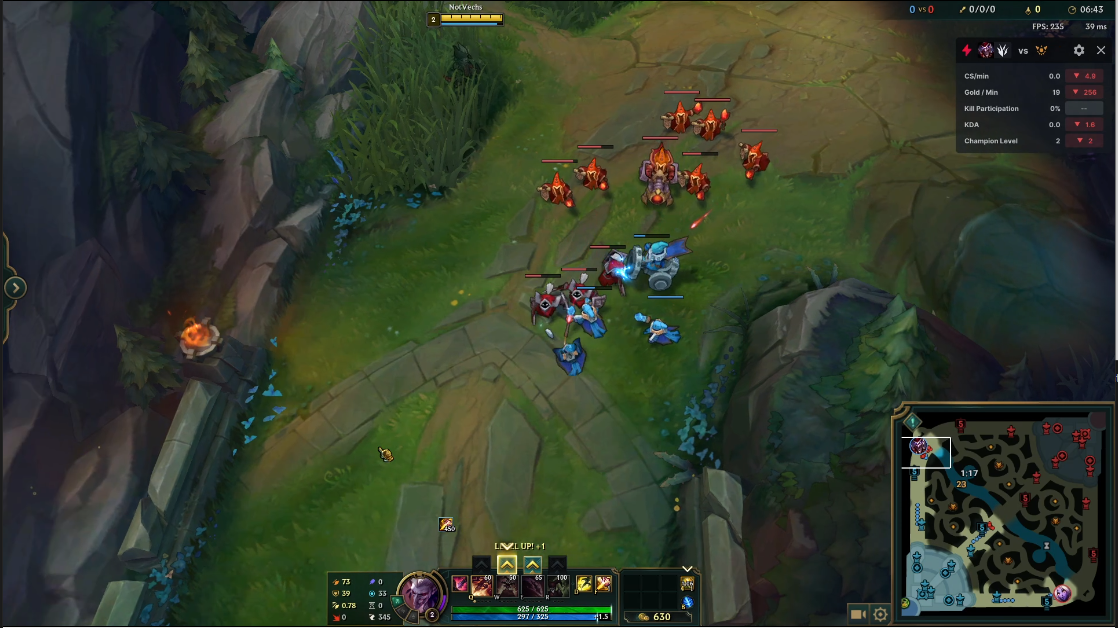
\includegraphics[width=\textwidth]{Crash.PNG}
\caption[A duck]{z}
so yeah

\end{table}


\newpage
\section{"Playing" with the Results}
fun words

\end{document}